\lstinputlisting[language=bash,basicstyle=\small]{python_codes/fieldstone_97/keywords}

\begin{center}
Code at \url{https://github.com/cedrict/fieldstone/tree/master/python_codes/fieldstone_97}
\end{center}

\par\noindent\rule{\textwidth}{0.4pt}

%%%%%%%%%%%%%%%%%%%%%%%%%%%%%%%%%%%%%%%%%%%%%%%%%%%%%%%%%%%%%%%%%%%%%%%%%%%%%%%%%%%%%%%%

All CRUST 1.0 data are available at \url{https://igppweb.ucsd.edu/~gabi/crust1.html}. 
The files {\tt crust1.rho} and {\tt crust1.bnds} count 64,800 lines,
corresponding to 360x180 points, i.e. a 1\si{\degree} resolution. 

As explained on the website: 
"The model is defined from 89.5 to -89.5 deg latitude (so that 
in fact the data is the co-latitude) and -179.5 to 179.5 deg
longitude. Longitudes are the inner loop, i.e. all longitudes are stored
for each latitude, then the next latitude is given. The model starts at 
89.5 N and 179.5 W."

The structure of the CRUST 1.0 data is as follows:

\begin{verbatim}
===========================================================
 crust1.rho | layer | name             | crust1.bnds
 --------------------------------------|----1-------
 1          | 1     | water            |
 --------------------------------------|----2-------
 2          | 2     | ice              |
 --------------------------------------|----3-------
 3          | 3     | upper sediments  |
 --------------------------------------|----4-------
 4          | 4     | mid sediments    |
 --------------------------------------|----5-------
 5          | 5     | lower sediments  | 
 --------------------------------------|----6-------
 6          | 6     | upper crust      |
 --------------------------------------|----7-------
 7          | 7     | mid crust        |
 --------------------------------------|----8-------
 8          | 8     | lower crust      |
 --------------------------------------|----9-------MOHO
 9          | 9
===========================================================
\end{verbatim}

This stone allows the user to choose a minimum and maximum radius, as well as a 
number of shells in between {\tt nrad}, and rewrites the data in spherical coordinates 
as the ascii file {\tt crust1p0\_full\_for\_aspect.ascii} which is in the format that \aspect{} expects.
Another file, {\tt crust1p0\_moho\_for\_aspect.ascii}, is produced. Its structure and intent
is similar to the first one, except that points above the moho are assigned a single 
density $\rho=2900\si{\kilo\gram\per\cubic\metre}$ while points below the 
moho are assigned $\rho=3300\si{\kilo\gram\per\cubic\metre}$.

Very importantly, \aspect{} does not read in densities bu temperatures. This stone then 
converts the density values into temperature using the simple relationship
\[
\rho = \rho_0 (1-\alpha(T-T_0))
\qquad \text{or,} \qquad
T= \frac{1}{\alpha} \left(1 - \frac{\rho}{\rho_0} \right)
\]
and we here take $\alpha = 3\cdot 10^{-5}\si{\per\kelvin}$, 
$T_0=0\si{\kelvin}$ and $\rho_0=3300\si{\kilo\gram\per\cubic\metre}$. 
This temperature is meaningless, but when used in the material model of \aspect{}, 
it yields the expected density field. 

CRUST 1.0 also comes with the file {\tt depthtomoho.xyz} which name is 
self-explanatory. Values are stored at coordinates $x.5$, $y.5$ (with $x\in[0,359]$
and $y\in [-89:89]$) so I assign a 1x1degree cell around it and give the whole cell 
the associated depth.
The data is exported as vtu file. One is a 2D lat-lon map (the vertical 
elevation of the map follows the moho depth) named {\tt moho\_map.vtu}, the other is a 
spherical mesh where each cell is assigned the radius of the Erath minus the moho depth, 
named {\tt moho\_shell.vtu}.

\begin{center}
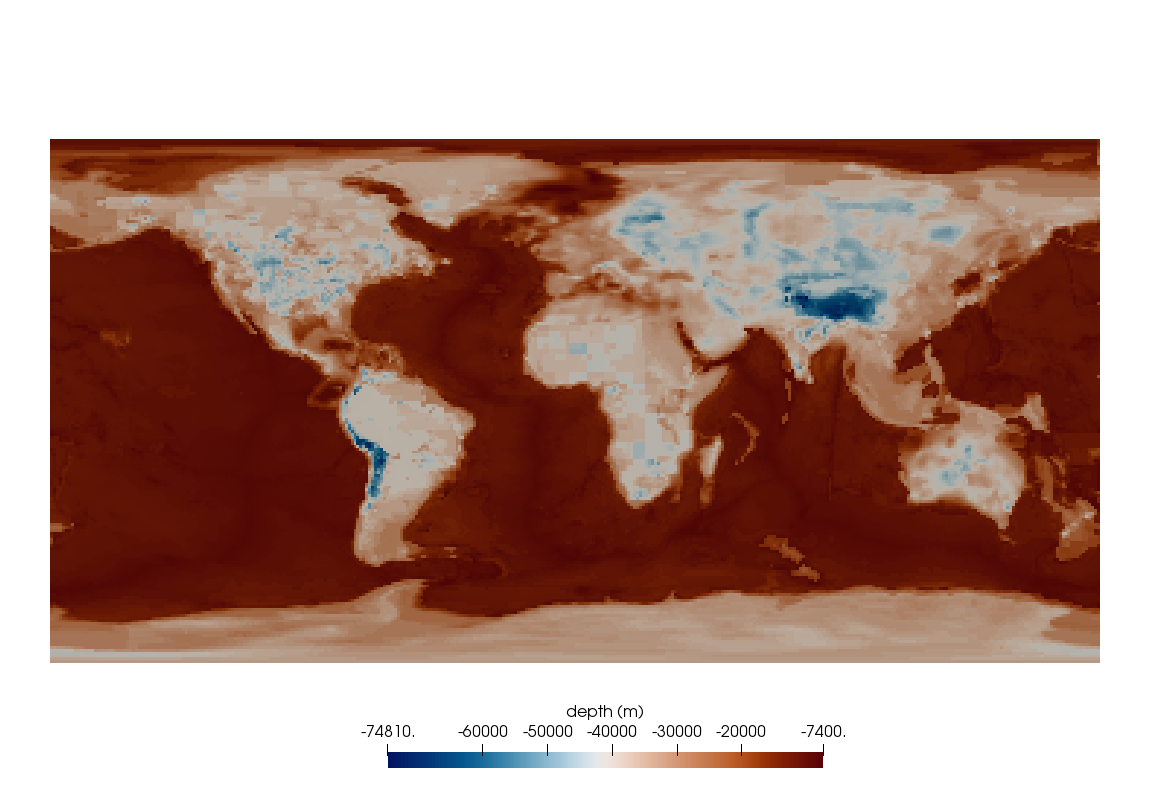
\includegraphics[width=7.cm]{python_codes/fieldstone_97/images/mohodepth1}
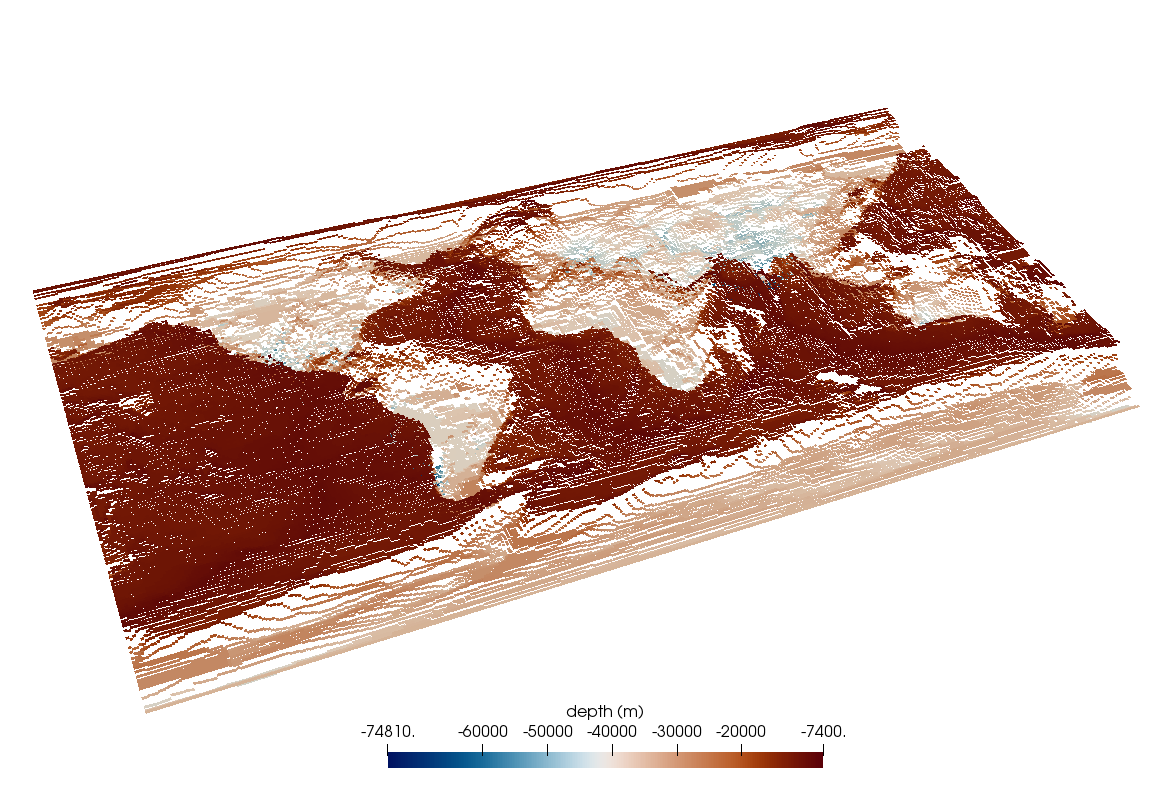
\includegraphics[width=7.cm]{python_codes/fieldstone_97/images/mohodepth2}\\
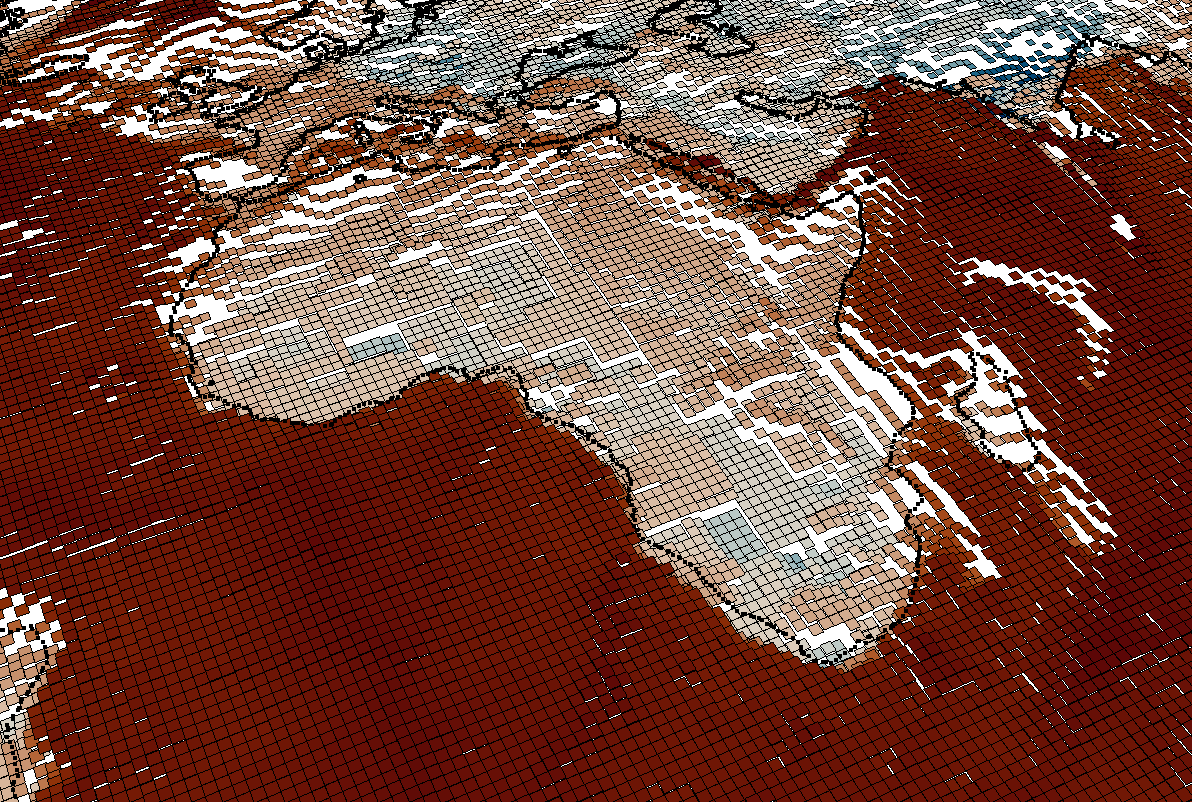
\includegraphics[width=7.cm]{python_codes/fieldstone_97/images/mohodepth7}
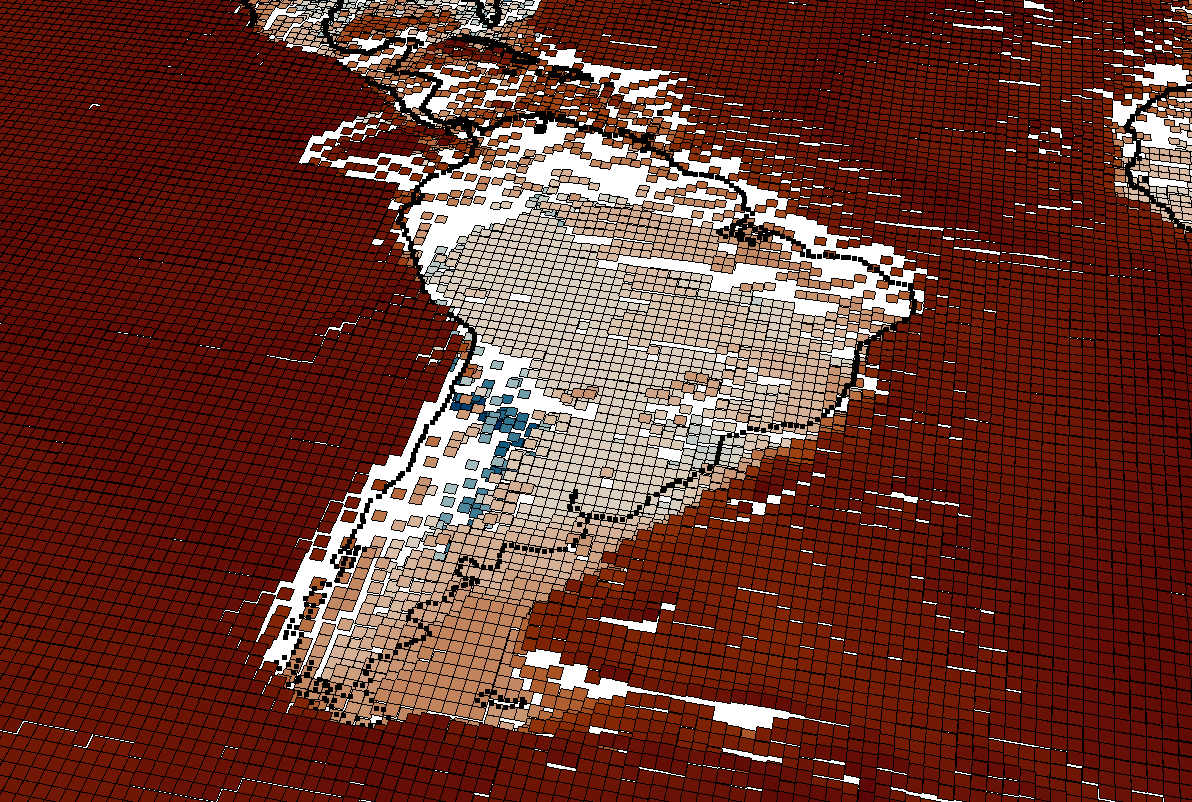
\includegraphics[width=7.cm]{python_codes/fieldstone_97/images/mohodepth8}\\
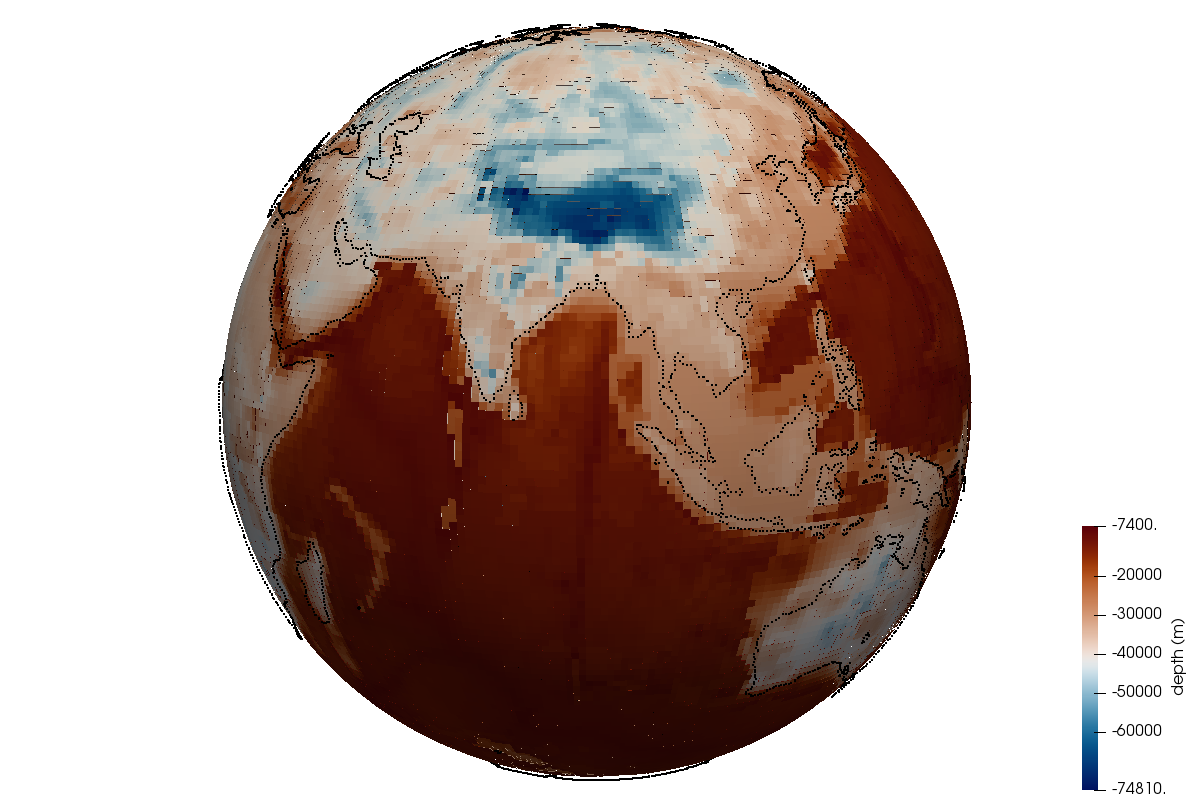
\includegraphics[width=7.cm]{python_codes/fieldstone_97/images/mohodepth3}
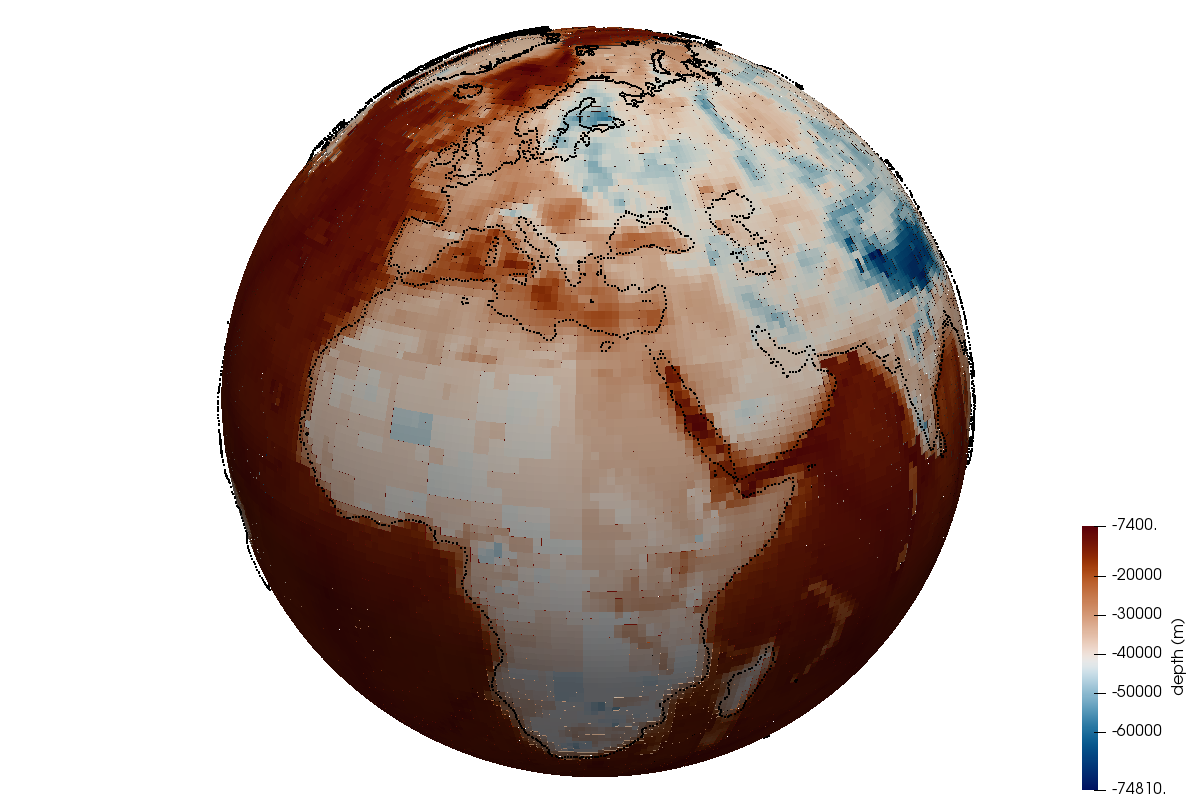
\includegraphics[width=7.cm]{python_codes/fieldstone_97/images/mohodepth4}\\
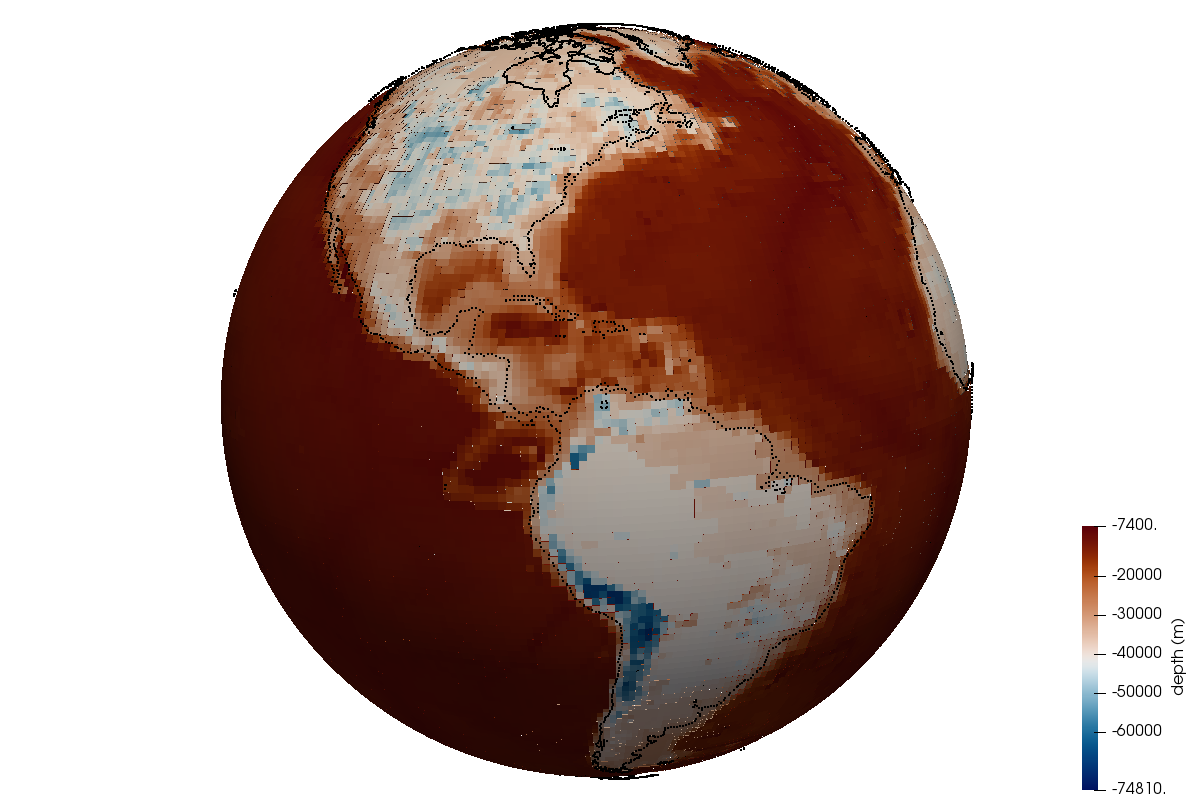
\includegraphics[width=7.cm]{python_codes/fieldstone_97/images/mohodepth5}
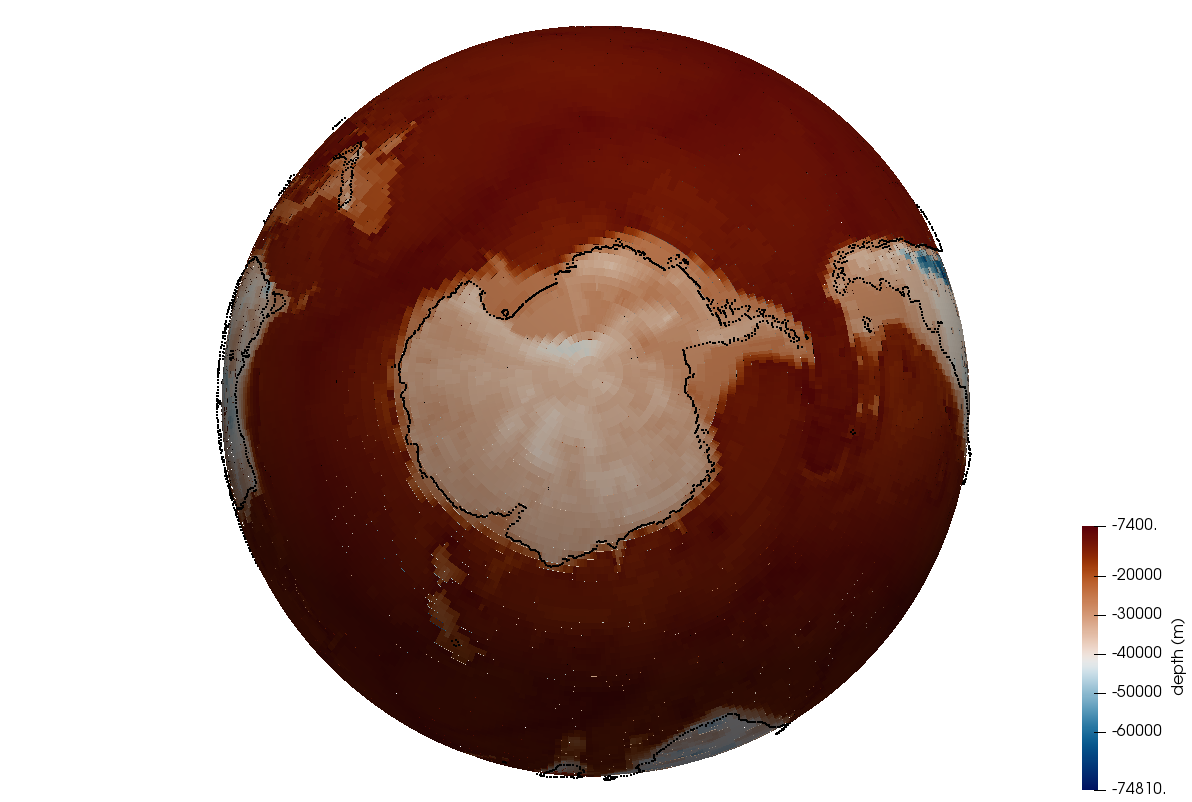
\includegraphics[width=7.cm]{python_codes/fieldstone_97/images/mohodepth6}\\
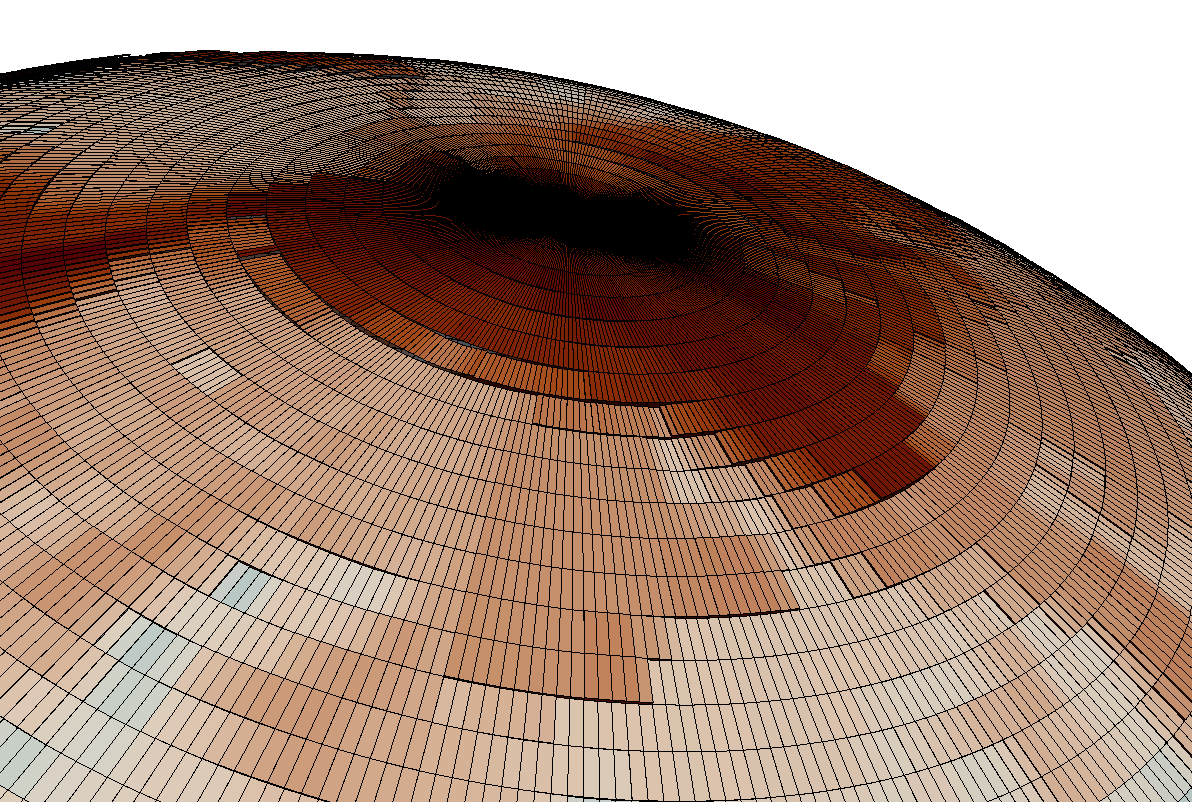
\includegraphics[width=7.cm]{python_codes/fieldstone_97/images/mohodepth9}
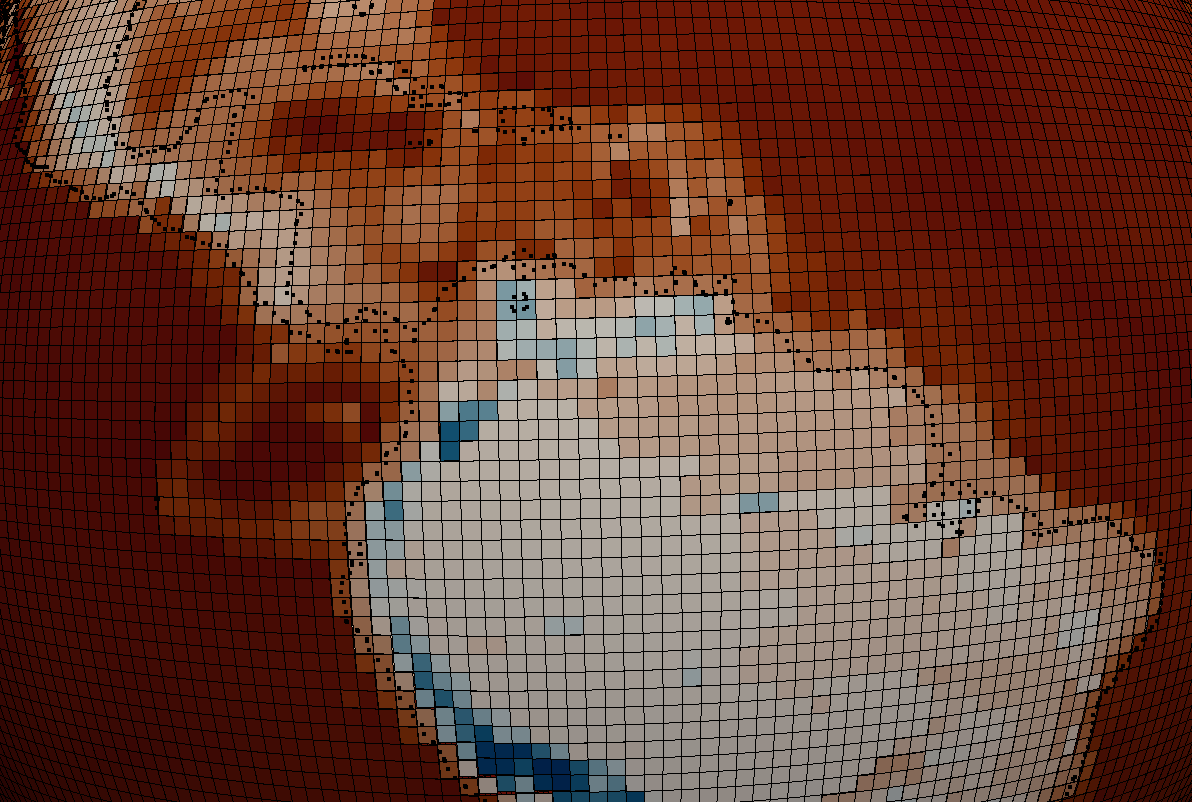
\includegraphics[width=7.cm]{python_codes/fieldstone_97/images/mohodepth10}\\
{\captionfont colormap=vik, see \url{http://www.fabiocrameri.ch/vik.php}.
Continent boundaries are from Stone 69.}
\end{center}
